\documentclass{standalone}
\usepackage{tikz}
\usetikzlibrary{patterns, positioning}


\begin{document}
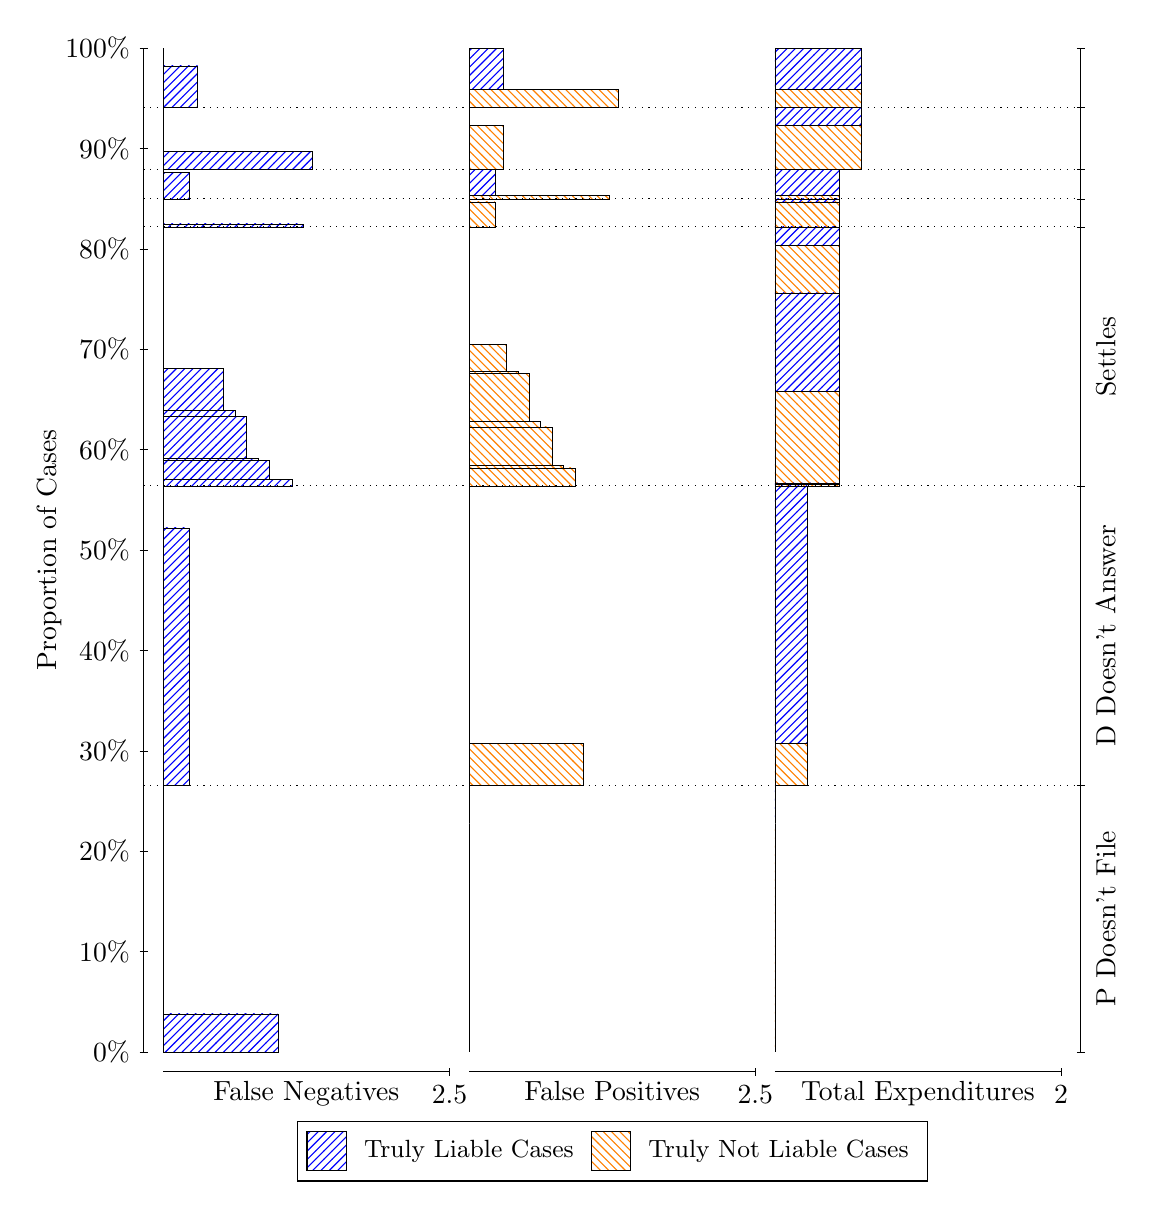
\begin{tikzpicture}
\draw[black, very thin] (1.5,1.75) -- (1.5,14.5);
\node[rotate=90, text=black, anchor=center] at (0.3, 8.125) {Proportion of Cases};
\draw[black, very thin] (1.45,1.75) -- (1.55,1.75);
\node[text=black, anchor=east] at (1.45, 1.75) {0\%};
\draw[black, very thin] (1.45,3.025) -- (1.55,3.025);
\node[text=black, anchor=east] at (1.45, 3.025) {10\%};
\draw[black, very thin] (1.45,4.3) -- (1.55,4.3);
\node[text=black, anchor=east] at (1.45, 4.3) {20\%};
\draw[black, very thin] (1.45,5.575) -- (1.55,5.575);
\node[text=black, anchor=east] at (1.45, 5.575) {30\%};
\draw[black, very thin] (1.45,6.85) -- (1.55,6.85);
\node[text=black, anchor=east] at (1.45, 6.85) {40\%};
\draw[black, very thin] (1.45,8.125) -- (1.55,8.125);
\node[text=black, anchor=east] at (1.45, 8.125) {50\%};
\draw[black, very thin] (1.45,9.4) -- (1.55,9.4);
\node[text=black, anchor=east] at (1.45, 9.4) {60\%};
\draw[black, very thin] (1.45,10.675) -- (1.55,10.675);
\node[text=black, anchor=east] at (1.45, 10.675) {70\%};
\draw[black, very thin] (1.45,11.95) -- (1.55,11.95);
\node[text=black, anchor=east] at (1.45, 11.95) {80\%};
\draw[black, very thin] (1.45,13.225) -- (1.55,13.225);
\node[text=black, anchor=east] at (1.45, 13.225) {90\%};
\draw[black, very thin] (1.45,14.5) -- (1.55,14.5);
\node[text=black, anchor=east] at (1.45, 14.5) {100\%};

\draw[black, very thin] (13.4,1.75) -- (13.4,14.5);
\draw[black, very thin] (13.35,1.75) -- (13.45,1.75);
\node[anchor=west] at (13.35, 1.75) {};
\draw[black, very thin] (13.35,5.1379) -- (13.45,5.1379);
\node[anchor=west] at (13.35, 5.1379) {};
\draw[black, very thin] (13.35,8.9389) -- (13.45,8.9389);
\node[anchor=west] at (13.35, 8.9389) {};
\draw[black, very thin] (13.35,12.229) -- (13.45,12.229);
\node[anchor=west] at (13.35, 12.229) {};
\draw[black, very thin] (13.35,12.584) -- (13.45,12.584);
\node[anchor=west] at (13.35, 12.584) {};
\draw[black, very thin] (13.35,12.957) -- (13.45,12.957);
\node[anchor=west] at (13.35, 12.957) {};
\draw[black, very thin] (13.35,13.745) -- (13.45,13.745);
\node[anchor=west] at (13.35, 13.745) {};
\draw[black, very thin] (13.35,14.5) -- (13.45,14.5);
\node[anchor=west] at (13.35, 14.5) {};

\draw[black, very thin, pattern color=blue, pattern=north east lines] (1.75,1.75) rectangle (3.2033,2.2339);
\draw[black, very thin, pattern color=orange, pattern=north west lines] (1.75,2.2339) rectangle (1.75,5.1379);
\draw[black, very thin, pattern color=blue, pattern=north east lines] (1.75,5.1379) rectangle (2.077,8.4063);
\draw[black, very thin, pattern color=orange, pattern=north west lines] (1.75,8.4063) rectangle (1.75,8.9389);
\draw[black, very thin, pattern color=blue, pattern=north east lines] (1.75,8.9389) rectangle (3.385,9.0202);
\draw[black, very thin, pattern color=blue, pattern=north east lines] (1.75,9.0202) rectangle (3.2397,9.0261);
\draw[black, very thin, pattern color=blue, pattern=north east lines] (1.75,9.0261) rectangle (3.0943,9.2582);
\draw[black, very thin, pattern color=blue, pattern=north east lines] (1.75,9.2582) rectangle (2.949,9.2934);
\draw[black, very thin, pattern color=blue, pattern=north east lines] (1.75,9.2934) rectangle (2.8037,9.8261);
\draw[black, very thin, pattern color=blue, pattern=north east lines] (1.75,9.8261) rectangle (2.6583,9.8948);
\draw[black, very thin, pattern color=blue, pattern=north east lines] (1.75,9.8948) rectangle (2.513,10.436);
\draw[black, very thin, pattern color=orange, pattern=north west lines] (1.75,10.436) rectangle (1.75,12.229);
\draw[black, very thin, pattern color=blue, pattern=north east lines] (1.75,12.229) rectangle (3.5303,12.266);
\draw[black, very thin, pattern color=orange, pattern=north west lines] (1.75,12.266) rectangle (1.75,12.584);
\draw[black, very thin, pattern color=blue, pattern=north east lines] (1.75,12.584) rectangle (2.077,12.917);
\draw[black, very thin, pattern color=orange, pattern=north west lines] (1.75,12.917) rectangle (1.75,12.957);
\draw[black, very thin, pattern color=blue, pattern=north east lines] (1.75,12.957) rectangle (3.6393,13.184);
\draw[black, very thin, pattern color=orange, pattern=north west lines] (1.75,13.184) rectangle (1.75,13.745);
\draw[black, very thin, pattern color=blue, pattern=north east lines] (1.75,13.745) rectangle (2.186,14.273);
\draw[black, very thin, pattern color=orange, pattern=north west lines] (1.75,14.273) rectangle (1.75,14.5);
\draw[black, very thin, pattern color=orange, pattern=north west lines] (5.6333,1.75) rectangle (5.6333,4.654);
\draw[black, very thin, pattern color=blue, pattern=north east lines] (5.6333,4.654) rectangle (5.6333,5.1379);
\draw[black, very thin, pattern color=orange, pattern=north west lines] (5.6333,5.1379) rectangle (7.0867,5.6705);
\draw[black, very thin, pattern color=blue, pattern=north east lines] (5.6333,5.6705) rectangle (5.6333,8.9389);
\draw[black, very thin, pattern color=orange, pattern=north west lines] (5.6333,8.9389) rectangle (6.9777,9.1669);
\draw[black, very thin, pattern color=orange, pattern=north west lines] (5.6333,9.1669) rectangle (6.8323,9.199);
\draw[black, very thin, pattern color=orange, pattern=north west lines] (5.6333,9.199) rectangle (6.687,9.6884);
\draw[black, very thin, pattern color=orange, pattern=north west lines] (5.6333,9.6884) rectangle (6.5417,9.7556);
\draw[black, very thin, pattern color=orange, pattern=north west lines] (5.6333,9.7556) rectangle (6.3963,10.364);
\draw[black, very thin, pattern color=orange, pattern=north west lines] (5.6333,10.364) rectangle (6.251,10.392);
\draw[black, very thin, pattern color=orange, pattern=north west lines] (5.6333,10.392) rectangle (6.1057,10.732);
\draw[black, very thin, pattern color=blue, pattern=north east lines] (5.6333,10.732) rectangle (5.6333,12.229);
\draw[black, very thin, pattern color=orange, pattern=north west lines] (5.6333,12.229) rectangle (5.9603,12.547);
\draw[black, very thin, pattern color=blue, pattern=north east lines] (5.6333,12.547) rectangle (5.6333,12.584);
\draw[black, very thin, pattern color=orange, pattern=north west lines] (5.6333,12.584) rectangle (7.4137,12.624);
\draw[black, very thin, pattern color=blue, pattern=north east lines] (5.6333,12.624) rectangle (5.9603,12.957);
\draw[black, very thin, pattern color=orange, pattern=north west lines] (5.6333,12.957) rectangle (6.0693,13.518);
\draw[black, very thin, pattern color=blue, pattern=north east lines] (5.6333,13.518) rectangle (5.6333,13.745);
\draw[black, very thin, pattern color=orange, pattern=north west lines] (5.6333,13.745) rectangle (7.5227,13.972);
\draw[black, very thin, pattern color=blue, pattern=north east lines] (5.6333,13.972) rectangle (6.0693,14.5);
\draw[black, very thin, pattern color=orange, pattern=north west lines] (9.5167,1.75) rectangle (9.5167,4.654);
\draw[black, very thin, pattern color=blue, pattern=north east lines] (9.5167,4.654) rectangle (9.5167,5.1379);
\draw[black, very thin, pattern color=orange, pattern=north west lines] (9.5167,5.1379) rectangle (9.9254,5.6705);
\draw[black, very thin, pattern color=blue, pattern=north east lines] (9.5167,5.6705) rectangle (9.9254,8.9389);
\draw[black, very thin, pattern color=orange, pattern=north west lines] (9.5167,8.9389) rectangle (10.334,8.962);
\draw[black, very thin, pattern color=blue, pattern=north east lines] (9.5167,8.962) rectangle (10.334,8.9763);
\draw[black, very thin, pattern color=orange, pattern=north west lines] (9.5167,8.9763) rectangle (10.334,10.138);
\draw[black, very thin, pattern color=blue, pattern=north east lines] (9.5167,10.138) rectangle (10.334,11.389);
\draw[black, very thin, pattern color=orange, pattern=north west lines] (9.5167,11.389) rectangle (10.334,11.997);
\draw[black, very thin, pattern color=blue, pattern=north east lines] (9.5167,11.997) rectangle (10.334,12.229);
\draw[black, very thin, pattern color=orange, pattern=north west lines] (9.5167,12.229) rectangle (10.334,12.547);
\draw[black, very thin, pattern color=blue, pattern=north east lines] (9.5167,12.547) rectangle (10.334,12.584);
\draw[black, very thin, pattern color=orange, pattern=north west lines] (9.5167,12.584) rectangle (10.334,12.624);
\draw[black, very thin, pattern color=blue, pattern=north east lines] (9.5167,12.624) rectangle (10.334,12.957);
\draw[black, very thin, pattern color=orange, pattern=north west lines] (9.5167,12.957) rectangle (10.607,13.518);
\draw[black, very thin, pattern color=blue, pattern=north east lines] (9.5167,13.518) rectangle (10.607,13.745);
\draw[black, very thin, pattern color=orange, pattern=north west lines] (9.5167,13.745) rectangle (10.607,13.972);
\draw[black, very thin, pattern color=blue, pattern=north east lines] (9.5167,13.972) rectangle (10.607,14.5);
\draw[black, dotted] (1.5,5.1379) -- (13.4,5.1379);
\draw[black, dotted] (1.5,8.9389) -- (13.4,8.9389);
\draw[black, dotted] (1.5,12.229) -- (13.4,12.229);
\draw[black, dotted] (1.5,12.584) -- (13.4,12.584);
\draw[black, dotted] (1.5,12.957) -- (13.4,12.957);
\draw[black, dotted] (1.5,13.745) -- (13.4,13.745);
\draw[black, very thin] (1.75,1.5) -- (5.3833,1.5);
\node[text=black, anchor=north] at (3.5667, 1.5) {False Negatives};
\draw[black, very thin] (5.3833,1.45) -- (5.3833,1.55);
\node[text=black, anchor=north] at (5.3833, 1.45) {2.5};

\draw[black, very thin] (5.6333,1.5) -- (9.2667,1.5);
\node[text=black, anchor=north] at (7.45, 1.5) {False Positives};
\draw[black, very thin] (9.2667,1.45) -- (9.2667,1.55);
\node[text=black, anchor=north] at (9.2667, 1.45) {2.5};

\draw[black, very thin] (9.5167,1.5) -- (13.15,1.5);
\node[text=black, anchor=north] at (11.333, 1.5) {Total Expenditures};
\draw[black, very thin] (13.15,1.45) -- (13.15,1.55);
\node[text=black, anchor=north] at (13.15, 1.45) {2};

\node[text=black, centered, rotate=90] at (13.72, 3.4439) {P Doesn't File};
\node[text=black, centered, rotate=90] at (13.72, 7.0384) {D Doesn't Answer};
\node[text=black, centered, rotate=90] at (13.72, 10.584) {Settles};





\draw (7.449999999999999,1.5) node[draw=none] (baseCoordinate) {};
\begin{scope}[align=center]
        \matrix[scale=0.5, draw=black, below=0.5cm of baseCoordinate, nodes={draw}, column sep=0.1cm]{
            \node[rectangle, draw, minimum width=0.5cm, minimum height=0.5cm, pattern color=blue, pattern=north east lines] {}; &
            \node[draw=none, font=\small, text=black] (B) {Truly Liable Cases}; &
            \node[rectangle, draw, minimum width=0.5cm, minimum height=0.5cm, pattern color=orange, pattern=north west lines] {}; &
            \node[draw=none, font=\small, text=black] (B) {Truly Not Liable Cases}; \\
            };
\end{scope}

\end{tikzpicture}
\end{document}